\section{Ergebnisse}
Zunächst wurden bei einer Belichtungszeit von 30 Sekunden dark frames bei verschiedenen Temperaturen des Chips aufgenommen, um die ideale Betriebstemperatur des CCD zu ermitteln. Hierbei ergaben sich die in Tabelle \ref{tbl:adu_temp} dargestellten Werte, welche in Abb. \ref{fig:adu_temp} graphisch dargestellt sind. 
\begin{figure}[h!]
        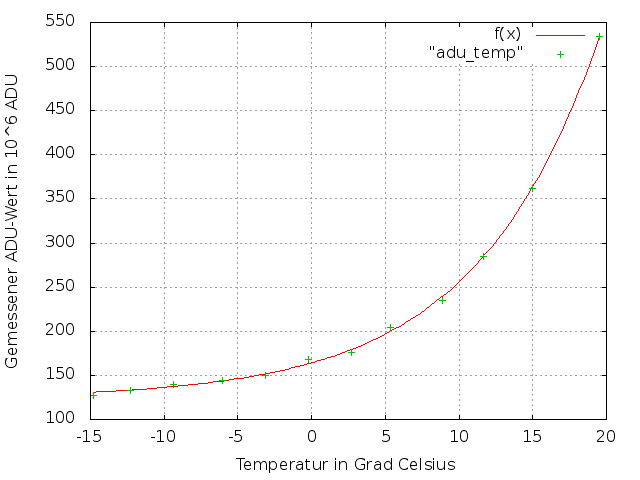
\includegraphics[width=.9\textwidth]{plot_adu_temp2.png}
\caption{ Auftragung von Dunkelstrom über der CCD-Temperatur }
\label{fig:adu_temp}
\end{figure}
Hier wurde der Verlauf mit einer Exponentialfunktion $f(T) = a \cdot \exp(T \cdot c) + b$ gefittet, welche theoretisch zu erwarten ist, da die Energie der Elektronen im Halbleiter prinzipiell boltzmann-verteilt ist. \\
Es ergibt sich also eine ideale Temperatur von etwa -15 $^\circ$ C im betrachteten Intervall von -15 bis + 20 $^\circ$ C. Eine tiefere Temperatur ist aufgrund der begrenzten Kühlleistung des CCD-Chips nicht erreichbar. Für die Fitparameter ergibt sich: 
$a = 40.0\  \mathrm{adu}, c = 0.119 \frac{1}{\mathrm{K}}, b = 124.2 \ \mathrm{adu}$. \\
Die Aufnahme eines bias frames bei einer Belichtungszeit von 0.12 s und einer Blendenöffnung von 5.6 wird in Abb. \ref{fig:bias} dargestellt. 
\begin{figure}[h!]
        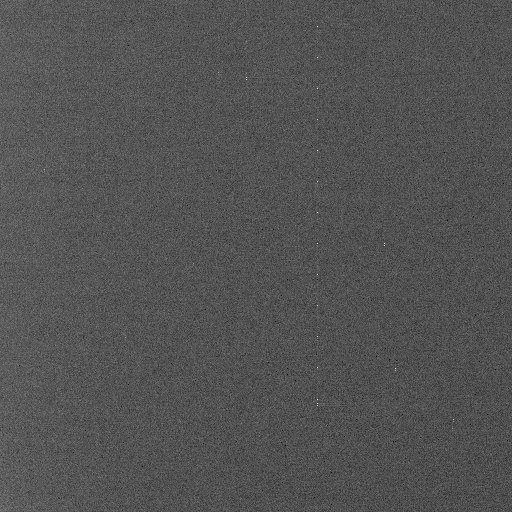
\includegraphics[width=.9\textwidth]{beiers_01.png}
\caption{ Aufnahme eines bias frame }
\label{fig:bias}
\end{figure}
Neben dem Rauschen im Hintergrund erkennt man mehrere senkrechte gepunktete Linien. Diese sind auf ein hot pixel in der entsprechenden Spalte zurückzuführen. Aufgrund des \enquote{schubweisen} Auslesens der Zeilen, welches  laut dem Betreuer durch Speichervorgänge in der Ausleseelektronik verursacht wird, kommt es in regelmäßigen zeitlichen Abständen zu einer Verzögerung beim Auslesen und somit zu hellen Punkten mit räumlich gleichem Abstand. Des weiteren ist ein leichter Helligkeitsgradient von links nach rechts sichtbar. Der Grund hierfür ist wahrscheinlich ein Temperaturgradient im CCD-Chip und ein somit räumlich unterschiedlicher Dunkelstrom. \\
Es wurden insgesamt 11 bias frames aufgenommen, deren mittlerer ADU-Wert sich zu 115.6 $ \pm 1.07$ ergibt. \\
Damit auch bei maximaler Belichtungszeit kein ueberbelichtetes Bild aufgenommen wurde, musste insgesamt ein Filter der Straerke 2048, der also nur $\frac{1}{2048}$ des Lichts transmittiert, verwendet werden. 
Zur Bestimmung des Gain-Faktors werden zu jeder Belichtungsdauer je zwei flat fields aufgenommen und ausgewertet. Dabei ergeben sich mit der Formel ... die in Tabelle \ref{tbl:gain} dargestellten Werte. Als gemittelter Wert ergibt sich 
\begin{equation}
\bar{g} = 1.940 \pm 0.04 \ \frac{\mathrm{adu}}{\mathrm{e}}. 
\end{equation}
Die Werte für den Gain-Faktor sind zwar alle im gleichen Bereich, es ist eine leichte Tendenz zu kleineren Gain-Faktoren bei groesseren Belichtungszeiten erkennbar. Der Grund hierfuer duerfte in Fehlern, die sich in der statistischen Betrachtung zur Herleitung der Formel fuer den Gain-Faktor ergeben, liegen. \\
In Tabelle \ref{tbl:adu_int} sind die Werte für gemessenen ADU-Werte aufgetragen über dem durch die Filter transmittierten Licht als Anteil der Lichtintensität vor dem Filter. \
Plottet man die ermittelten Werte, so ergibt sich der in \ref{plot:adu_int} dargestellte Verlauf. Werden die Datenpunkte mit der Funktion 
\begin{equation}
f(x) = a \cdot x + b
\end{equation}
gefittet, so ergeben sich die Werte $a = (119 \pm 5.0) \cdot 10^6 \ adu$ und $b = (2.8 \pm 1.4) \cdot 10^6 \ adu$.
\begin{figure}[h!]
        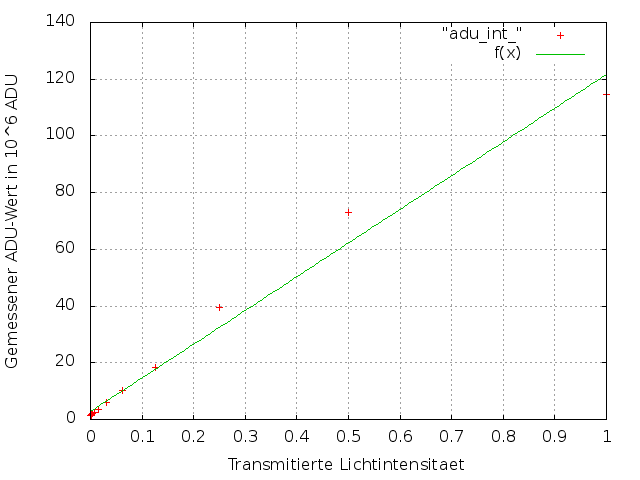
\includegraphics[width=.9\textwidth]{adu_int_.png}
\caption{ Auftragung des gemessenen ADU-Wertes ueber der einfallenden Lichtintensitaet }
\label{plot:adu_int}
\end{figure}
Problematisch ist, dass die Gerade die Punkte nahe der Null gut approximiert, die Werte mit groesserer Lichtintensitaet aber verfehlt. Grund hierfuer ist die grosse Anzahl an Punkten nahe der Null, die folglich den Fit dominieren. \\
Schliesslich wurden wurden die Effekte \enquote{smear} und \enquote{blooming} untersucht. 

\begin{figure}[h!]
        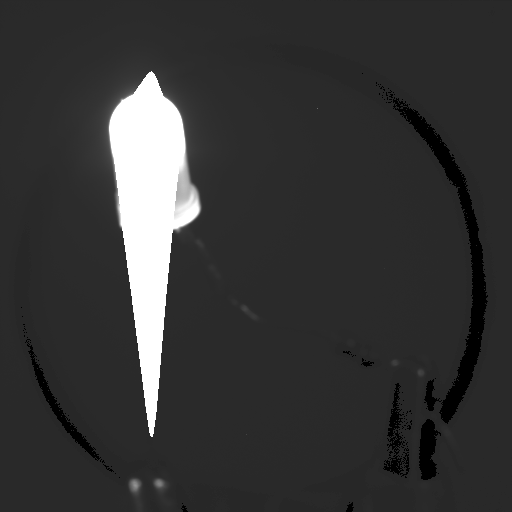
\includegraphics[width=.4\textwidth]{blooming.png}
\caption{ Aufnahme der Diode bei extremer Ueberbelichtung }
\label{fig:blooming}
\end{figure}
In \ref{fig:blooming} ist eine Aufnahme der Diode bei starker Ueberbelichtung dargestellt, was durch eine Belichtungszeit von 5 Sekudnen und einer Blende von 8f erreicht wurde. Man erkennt, dass nicht nur die tatsaechlich ueberbelichteten Pixel hell sind, sondern auch die spaltenweise benachbarten Pixel. Der Grund hierfuer ist, dass die Potentialtoepfe der einzelnen Pixel schlicht \enquote{ueberlaufen}, sodass Elektronen in benachbarte Pixel wandern. Dies geschieht vor allem innerhalb der Spalten und nur wenig in den Zeilen, da diese gegeneinander isoliert sind. Im Gegensatz dazu werden die Elektrnen in den Spalten verschoben, sodass diese nicht isoliert sein duerfen. \\ \\
Zur Veranschaulichung des Smear-Effektes wurden Aufnahmen bei deaktiviertem Shutter, einer Belichtungszeit von 0.5 Sekunden und ebenfalls einer Blende von 8f von gemacht, wobei der Strahlengang zunaechst durch ein Blatt Papier unterbrochen war, dass dann entfernt wurde. Die Ausleseelektronik befindet sich hier am oberen Bildrand. 
Bei der ersten Aufnahme zeigte sich das in \ref{fig:smear1} dargestellte Bild. 

\begin{figure}[h!]
        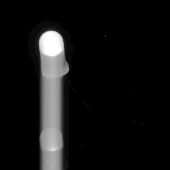
\includegraphics[width=.4\textwidth]{smear_unten_sebi.png}
\caption{ Erste Aufnahme nach Belichtungsbeginn }
\label{fig:smear1}
\end{figure}
Der Effekt erklaert sich folgendermassen:\\
Zu Beginn des Auslesens sind die ersten ausgelesenen Pixel unbelichtet. Wird das erste stark belichtete Pixel ausgelesen, so ergibt sich ein heller Punkt. Die nach diesem Pixel nachfolgenden Pixel werden waehrend dem zeitlich verzoegerten Auslesen weiter belichtet, sodass sie ueberhellt erscheinen. Diese Pixel liegen vom stark belichteten Pixel entgegen der Ausleserichtung. \\
Bei der zweiten Aufnahme ist dann ein durchgehender \enquote{smear} erkennbar, was daran liegt, dass die Pixel vor dem stark belichteten Pixel noch waerhend dem vorherhgehenden Ausleseprozess belichtet werden. Somit erscheint ein durchgehend heller Strich in der Spalte. Dies ist in Abb. \ref{fig:smear2} dargestellt. 

\begin{figure}[h!]
        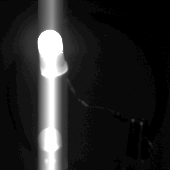
\includegraphics[width=.4\textwidth]{smear.png}
\caption{ Zweite Aufnahme }
\label{fig:smear2}
\end{figure}

Wird nun das Blatt Papier in den Strahlengang eingefuehrt, so ergibt sich die in Abb. \ref{fig:smear3} dargestellte Aufnahme. 

\begin{figure}[h!]
        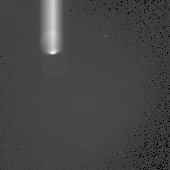
\includegraphics[width=.4\textwidth]{smear_oben_frueh.png}
\caption{ Aufnahme nach Einfuehren des Blattes }
\label{fig:smear3}
\end{figure}
Der Grund dafuer ist, dass die ersten Pixel wiederum waehrend dem vorherigen Auslesen belichtet werden und somit hell erscheinen. Nach dem EInfuehren des Blattes in den Strahlengang werden keine weiteren Pixel belichtet, sodass der helle Streifen an einer durch den Zeitpunkt des Einbringens des Blattes definierten Stelle abbricht. 
